% Generated from the public primitive catalog. Original Atlas drawing; Apache-2.0.
% Target: camellia-192; view: overview
\documentclass[border=9pt]{standalone}
% Original Atlas figure theme. Apache-2.0; see the repository LICENSE.
\usepackage[T1]{fontenc}
\usepackage{lmodern}
\usepackage{amsmath,amssymb}
\usepackage{tikz}
\usetikzlibrary{arrows.meta,positioning,calc,fit,backgrounds,decorations.pathreplacing,matrix}
\definecolor{atlasInk}{HTML}{172235}
\definecolor{atlasTeal}{HTML}{0D7B7D}
\definecolor{atlasMuted}{HTML}{637278}
\definecolor{atlasFill}{HTML}{EAF4F2}
\definecolor{atlasLine}{HTML}{B6C8C7}
\tikzset{
  every picture/.style={line width=.65pt,draw=atlasInk,>=Latex},
  every node/.style={text=atlasInk,font=\sffamily\small},
  box/.style={draw,rounded corners=1.5pt,minimum height=.9cm,minimum width=1.6cm,align=center,inner sep=6pt,fill=white},
  accent/.style={box,draw=atlasTeal,fill=atlasFill},
  wire/.style={->,line width=.7pt},
  keywire/.style={wire,draw=atlasTeal,dashed},
  xor/.style={draw,circle,fill=white,inner sep=0pt,minimum size=.38cm},
  add/.style={draw,rectangle,fill=white,inner sep=0pt,minimum size=.38cm},
  note/.style={font=\sffamily\scriptsize,text=atlasMuted,align=center},
  phase/.style={font=\sffamily\small\bfseries,text=atlasTeal},
  group/.style={draw=atlasLine,dashed,rounded corners=2pt,inner sep=8pt}
}
\newcommand{\rotl}{\mathbin{\lll}}
\newcommand{\rotr}{\mathbin{\ggg}}
\newcommand{\kx}{\operatorname{Keccak}\!\text{-}\!f[1600]}

\newcommand{\AtlasKeyBits}{192}
\newcommand{\AtlasKeyWords}{6}
\newcommand{\AtlasRounds}{24}
\newcommand{\AtlasPriorRounds}{23}
\newcommand{\AtlasRoundKeys}{25}
\newcommand{\AtlasDoubleRounds}{12}
\newcommand{\AtlasSixRoundGroups}{4}
\newcommand{\AtlasFLGroups}{3}
\newcommand{\AtlasRoundStart}{0}
\newcommand{\AtlasBlockBits}{128}
\newcommand{\AtlasOutputBits}{d}
\newcommand{\AtlasStateBits}{8w}
\newcommand{\AtlasNonceBits}{v}
\newcommand{\AtlasCounterBits}{q}
\newcommand{\AtlasStreamBlockBits}{b}
\newcommand{\AtlasRate}{r}
\newcommand{\AtlasCapacity}{c}
\newcommand{\AtlasSteps}{N}
\newcommand{\AtlasLastStep}{N-1}
\newcommand{\AtlasWordBits}{w}
\newcommand{\AtlasHashWords}{h}
\newcommand{\AtlasFeedForward}{\boxplus}
\newcommand{\AtlasByteOrder}{big-endian}
\newcommand{\AtlasDomain}{01}
\newif\ifAtlasXof
\AtlasXoffalse
\begin{document}
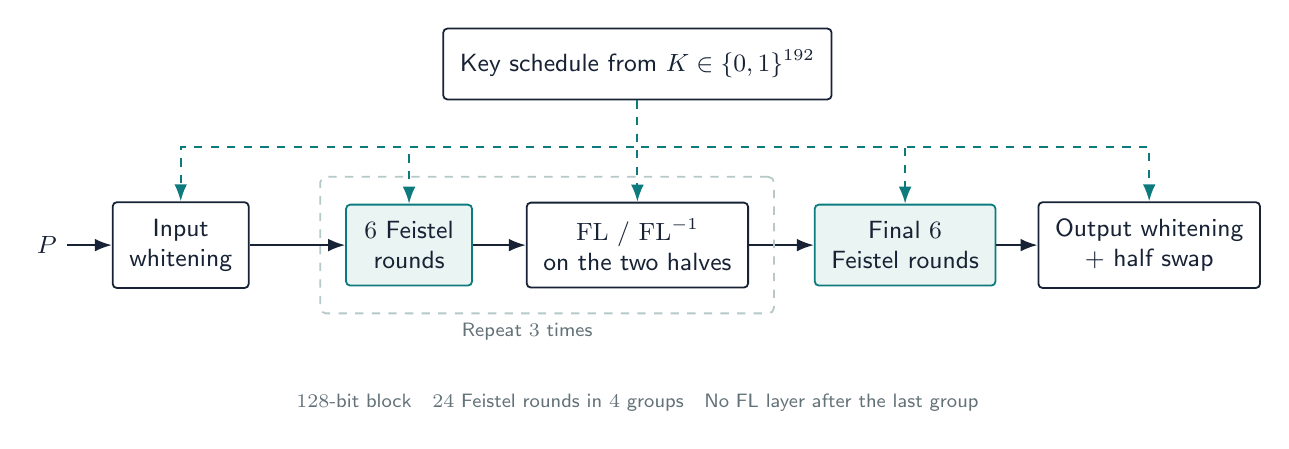
\begin{tikzpicture}
  \node (in) at (-.5,0) {$P$};
  \node[box] (pre) at (1.2,0) {Input\\whitening};
  \node[accent] (six) at (4.1,0) {$6$ Feistel\\rounds};
  \node[box] (fl) at (7,0) {$\mathrm{FL}$ / $\mathrm{FL}^{-1}$\\on the two halves};
  \node[accent] (last) at (10.4,0) {Final $6$\\Feistel rounds};
  \node[box] (post) at (13.5,0) {Output whitening\\$+$ half swap};
  \draw[wire] (in) -- (pre); \draw[wire] (pre) -- (six); \draw[wire] (six) -- (fl); \draw[wire] (fl) -- (last); \draw[wire] (last) -- (post);
  \node[group,fit=(six)(fl),inner sep=9pt] (repeat) {};
  \node[note] at (5.6,-1.1) {Repeat $\AtlasFLGroups$ times};
  \node[box] (schedule) at (7,2.3) {Key schedule from $K\in\{0,1\}^{\AtlasKeyBits}$};
  \foreach \target in {pre,six,fl,last,post} {\draw[keywire] (schedule.south) -- (7,1.25) -| (\target.north);}
  \node[note] at (7,-2) {$\AtlasBlockBits$-bit block\quad $\AtlasRounds$ Feistel rounds in $\AtlasSixRoundGroups$ groups\quad No FL layer after the last group};
\end{tikzpicture}

\end{document}
